\section{Introduction}
\label{sec:Introduction}

\begin{tcolorbox}[colback=brown!20!white, colframe=brown!20!white]

{\centering
\textit{"The first ultraintelligent machine is the last invention that man need ever make."}\par
}
\noindent\hfill--- \hyperlink{cite.good1966speculations}{I. J. Good (1966)}\par

\end{tcolorbox}

The development of artificial intelligence (AI) technology has driven a paradigm shift in agentic systems \citep{shoham1993agent, maes1994agents, wooldridge1995intelligent, yao2022react, Wang_2024}, from earlier narrow systems built around task-specific models or hand-engineered modules to modern agentic systems powered by \textbf{foundation models} (FMs), including large language models (LLMs) and vision-language models (VLMs), where natural language serves as a shared interface for representation, reasoning, and control.
Progress in foundation models has produced a qualitative shift in generalization, yielding striking successes across a wide range of domains, most notably code generation~\citep{chen2021evaluating}, language understanding~\citep{hendrycks2020measuring}, and mathematical and formal reasoning~\citep{wei2022chain}. These advances have brought a long-standing question to the foreground: the prospect of AI systems that improve themselves. Fundamentally, self-improvement is an inherently self-referential process. It defines a system's capacity to autonomously inspect, evaluate, and deliberately modify its own underlying optimization mechanisms and operational logic. Good articulated possible consequences of machine self-improvement~\citep{good1966speculations}, describing the possibility of an ``Intelligence Explosion'' once machines acquire the capacity to design more capable successors. Early work on concrete self-improvement algorithms dates back to Schmidhuber's self-referential learning framework~\citep{schmidhuber1987selfreferential}, which introduced mechanisms in which a system generates and evaluates modified descendant versions of itself. Establishing the theoretical ceiling of this pursuit, the G\"odel Machine \citep{schmidhuber2003godel} introduced a fully self-referential algorithm designed to rewrite its own code whenever it can mathematically prove an expected-utility improvement. While a persistent lineage of research successfully demonstrated neural networks (NNs) learning to program other networks via fast weights \citep{schmidhuber1992learning}, advancing to self-referential systems capable of modifying themselves \citep{schmidhuber1993self, irie2022modern}, and acting as meta-learning systems to discover their own learning algorithms \citep{hochreiter2001learning, schmidhuber2004optimal, kirsch2021meta, kirsch2022eliminating, irie2025metalearningcontinuallearningalgorithms}, parallel efforts introduced incremental self-improvement, establishing the ability to enforce long-term reward accelerations through the success-story algorithm for undoing policy self-modifications through backtracking \citep{Schmidhuber1994OnLH, schmidhuber1996simple, schmidhuber1997shifting}. However, scaling these visionary mechanisms into open-ended agents was historically constrained. Traditionally, systems were forced to search through vast, low-level spaces of assembly-like code or raw synaptic weights. Today, modern FMs alleviate this historical bottleneck by introducing natural language as a unified, highly capable semantic medium for reasoning, policy execution, and self-modification. By drastically reducing the search space for viable modifications, this language-native paradigm has drawn intense recent attention, with growing evidence demonstrating that FM-based self-improving agents can yield substantial empirical gains \citep{yuan2024self, acikgoz2025selfimprovingllmagentstesttime, qi2025webrl, zhang2025darwingodelmachineopenended}.


 To function autonomously in concrete environments, the FM serving as the cognitive core is typically enveloped by an operational {scaffold}, a structured framework comprising instruction schemes \citep{yuksekgonul2024textgradautomaticdifferentiationtext, guo2025evopromptconnectingllmsevolutionary}, memory systems \citep{chhikara2025mem0buildingproductionreadyai, zhang2026memrlselfevolvingagentsruntime}, tool interfaces \citep{qiu2025alitageneralistagentenabling, wölflein2025llmagentsmakingagent}, and control logic \citep{hong2023metagpt,10.5555/3692070.3694667,xiong2025beyond}. Recently, such an operational scaffold is often also referred to as an agent {harness} \citep{rajasekaran2026harnessdesign, trivedy2026agentharness, zhang2026selfharnessharnessesimprove, zhong2026aiharnessengineeringruntime}, while this survey uses the term scaffold to emphasize the modifiable structures surrounding the foundation model. Operationally, this scaffold acts as a controller that constructs context, selects actions, and enforces constraints. This modern architecture was conceptually foreshadowed by the "learning to think" framework \citep{schmidhuber2015learning}, where a general-purpose controller learned to dynamically query, or "prompt," a predictive world model to generate reasoning sequences akin to a modern "chain of thought" \citep{wei2022chain}.
Building upon this core-and-scaffold architecture, the integration of these classical control principles has crystallized into an emergent paradigm, which we refer to as FM-based self-improving agents. Because modern agentic systems comprise both the aforementioned neural core and scaffold, we organize this survey around a unified taxonomy with two primary pathways, as illustrated in Fig.~\ref{fig:mainfig} and summarized chronologically in Fig.~\ref{fig:agent_timeline}. The first pathway, which we call \textbf{foundation model improvement}, aims to achieve a slower but more stable form of long-term consolidation by updating the underlying model, thereby amortizing capability gains across varied tasks \citep{huang2023large, zhao2024selfguidebettertaskspecificinstruction, wang2025improvingmodelalignmentcollective, xiao2025uigenie, bougie2026alignuserhumanalignedllmagents}. The second pathway, which we call \textbf{scaffold improvement}, is typically faster and more easily reversible; it improves the agent by updating structural components, including prompts, memory, tool interfaces, and end-to-end control logic, to reshape the agent’s effective observation and action semantics \citep{fernando2024promptbreeder, chhikara2025mem0buildingproductionreadyai, wölflein2025llmagentsmakingagent, zhang2025darwingodelmachineopenended, borthwick2026robophdselfimprovingtexttosqlautonomous}. Although these pathways differ in their targets of modification, both are fundamentally driven by learning signals extracted during interaction. Accordingly, our taxonomy further refines these methods by separating \textit{what} is updated from \textit{where} the improvement signals originate, providing a common language for comparing disparate methods on a consistent footing. Fig.~\ref{fig:self_improving_taxonomy} provides a unified taxonomy of this survey.


% =================
\begin{wraptable}{r}{0.55\textwidth}
    \vspace{-\intextsep}
    \centering
    \footnotesize
    \setlength{\tabcolsep}{3pt}
    \renewcommand{\arraystretch}{1.08}
    \renewcommand{\tabularxcolumn}[1]{m{#1}}

    % --- compact badges (no extra packages needed beyond xcolor) ---
    \newcommand{\badgeC}{\textcolor{green!55!black}{\bfseries\cmark}}
    \newcommand{\badgeO}{\textcolor{orange!85!black}{\bfseries\omark}}
    \newcommand{\badgeN}{\textcolor{red!70!black}{\bfseries\nmark}}

    % zebra rows
    \rowcolors{3}{cyan!3}{white}

    \begin{tabularx}{\linewidth}{
        >{\columncolor{black!4}\hsize=2.25\hsize\raggedright\arraybackslash}X
        *{4}{>{\hsize=0.6875\hsize\centering\arraybackslash}X}
    }
    \toprule
    \rowcolor{cyan!8}
    \textbf{Dimension} & \textbf{Ours (2026)} & \citet{gao2025surveyselfevolvingagentspath} & \citet{fang2025comprehensivesurveyselfevolvingai} & \citet{tao2024surveyselfevolutionlargelanguage} \\
    \midrule
    
    \textbf{Agent formulation}     & \badgeC & \badgeC & \badgeC & \badgeO \\
    \textbf{Definition scope}       & \badgeC & \badgeC & \badgeO & \badgeO \\
    \textbf{Historical roots}     & \badgeC & \badgeN & \badgeO & \badgeO \\
    \textbf{Signal lens}            & \badgeC & \badgeO & \badgeC & \badgeC \\
    \textbf{Update substrate}       & \badgeC & \badgeC & \badgeC & \badgeO \\
    \textbf{Evaluation lens}        & \badgeC & \badgeC & \badgeC & \badgeC \\
    \textbf{Domain coverage}        & \badgeC & \badgeO & \badgeO & \badgeN \\
    \textbf{Outlook \& issues}      & \badgeC & \badgeO & \badgeC & \badgeO \\
    
    \bottomrule
    \end{tabularx}

    \vspace{2pt}
    {\scriptsize
    \textcolor{green!55!black}{\bfseries\cmark} primary \quad
    \textcolor{orange!85!black}{\bfseries\omark} secondary \quad
    \textcolor{red!70!black}{\bfseries\nmark} not focus
    }

    \caption{Comparison of organizing emphases across related surveys.}
    \vspace{-8pt}
    \label{tab:survey-compare}
\end{wraptable}
% =================

Despite the rapid proliferation of such empirical frameworks, the broader research landscape remains highly fragmented in both terminology and scope. Closely related ideas are often described under different labels (e.g., self-correction, meta-prompting, or self-play), obscuring underlying mechanistic similarities. Recent surveys have provided valuable perspectives by organizing self-evolving agents along dimensions such as what to evolve, when to evolve, and how to evolve \citep{gao2025surveyselfevolvingagentspath, fang2025comprehensivesurveyselfevolvingai}, or by focusing specifically on the autonomous learning capabilities of static LLMs \citep{tao2024surveyselfevolutionlargelanguage}. 
However, existing reviews often treat foundation model fine-tuning and agent scaffolding as isolated topics, lacking a unified formal perspective. Furthermore, few trace the conceptual roots of self-improvement back to classical AI. To bridge this gap, our survey provides a rigorous and systematic positioning of these modern agentic systems. We offer a comprehensive taxonomy under a unified formalization, clarifying their historical evolution and providing a clear, forward-looking roadmap for self-improvement. Concretely, our main contributions are as follows:
\begin{itemize}
    \item \textbf{Historical Context and Evolution.} We trace the evolutionary roots of self-improving systems from classical AI to modern FM-based agents, establishing a clear trajectory for how foundational learning mechanisms have adapted to the agentic era.
    \item \textbf{A Unified Formalization and Systematic Taxonomy.} Under our proposed formulation, we systematically categorize mechanisms into two distinct pathways: foundation model improvement and  scaffold improvement (covering prompt optimization, memory evolution, tool governance, and full-scaffold redesign).    
    \item \textbf{Empirical Landscape, Evaluation Paradigms, and Frontiers.} We integrate the classification system with practical applications (such as software engineering, web navigation, and scientific discovery) and critically analyze current evaluation protocols. By comparing mechanism-level benchmarking and end-to-end evaluation, we highlight the security factors and challenges that need to be considered in achieving reliable, continuous self-improvement.
\end{itemize}


The remainder of this survey is organized as follows. Section~\ref{sec:Historical_Context_and_Theoretical_Foundations} traces the historical context and theoretical foundations of self-improving systems. Section~\ref{sec:Definitions} introduces the systems view of foundation-model-based agents and formalizes the problem setting. Section~\ref{sec:A_Taxonomy_of_Self_Improvement_Mechanisms} presents our unified taxonomy, outlining the two primary pathways for improvement. These pathways are subsequently surveyed in depth: Section~\ref{sec:Foundation_Model_Improvement} covers updates to the underlying foundation model, while Section~\ref{sec:Scaffolding_Improvement} focuses on structural modifications to the surrounding scaffold. Section~\ref{sec:Applications} reviews practical instantiations across representative domains. Section~\ref{sec:Evaluation} discusses protocols and benchmarks for evaluating these systems. Finally, Section~\ref{sec:Discussion} synthesizes open problems and safety considerations, followed by concluding remarks in Section~\ref{sec:Conclusion}.


\begin{figure*}[ht]
    \centering
    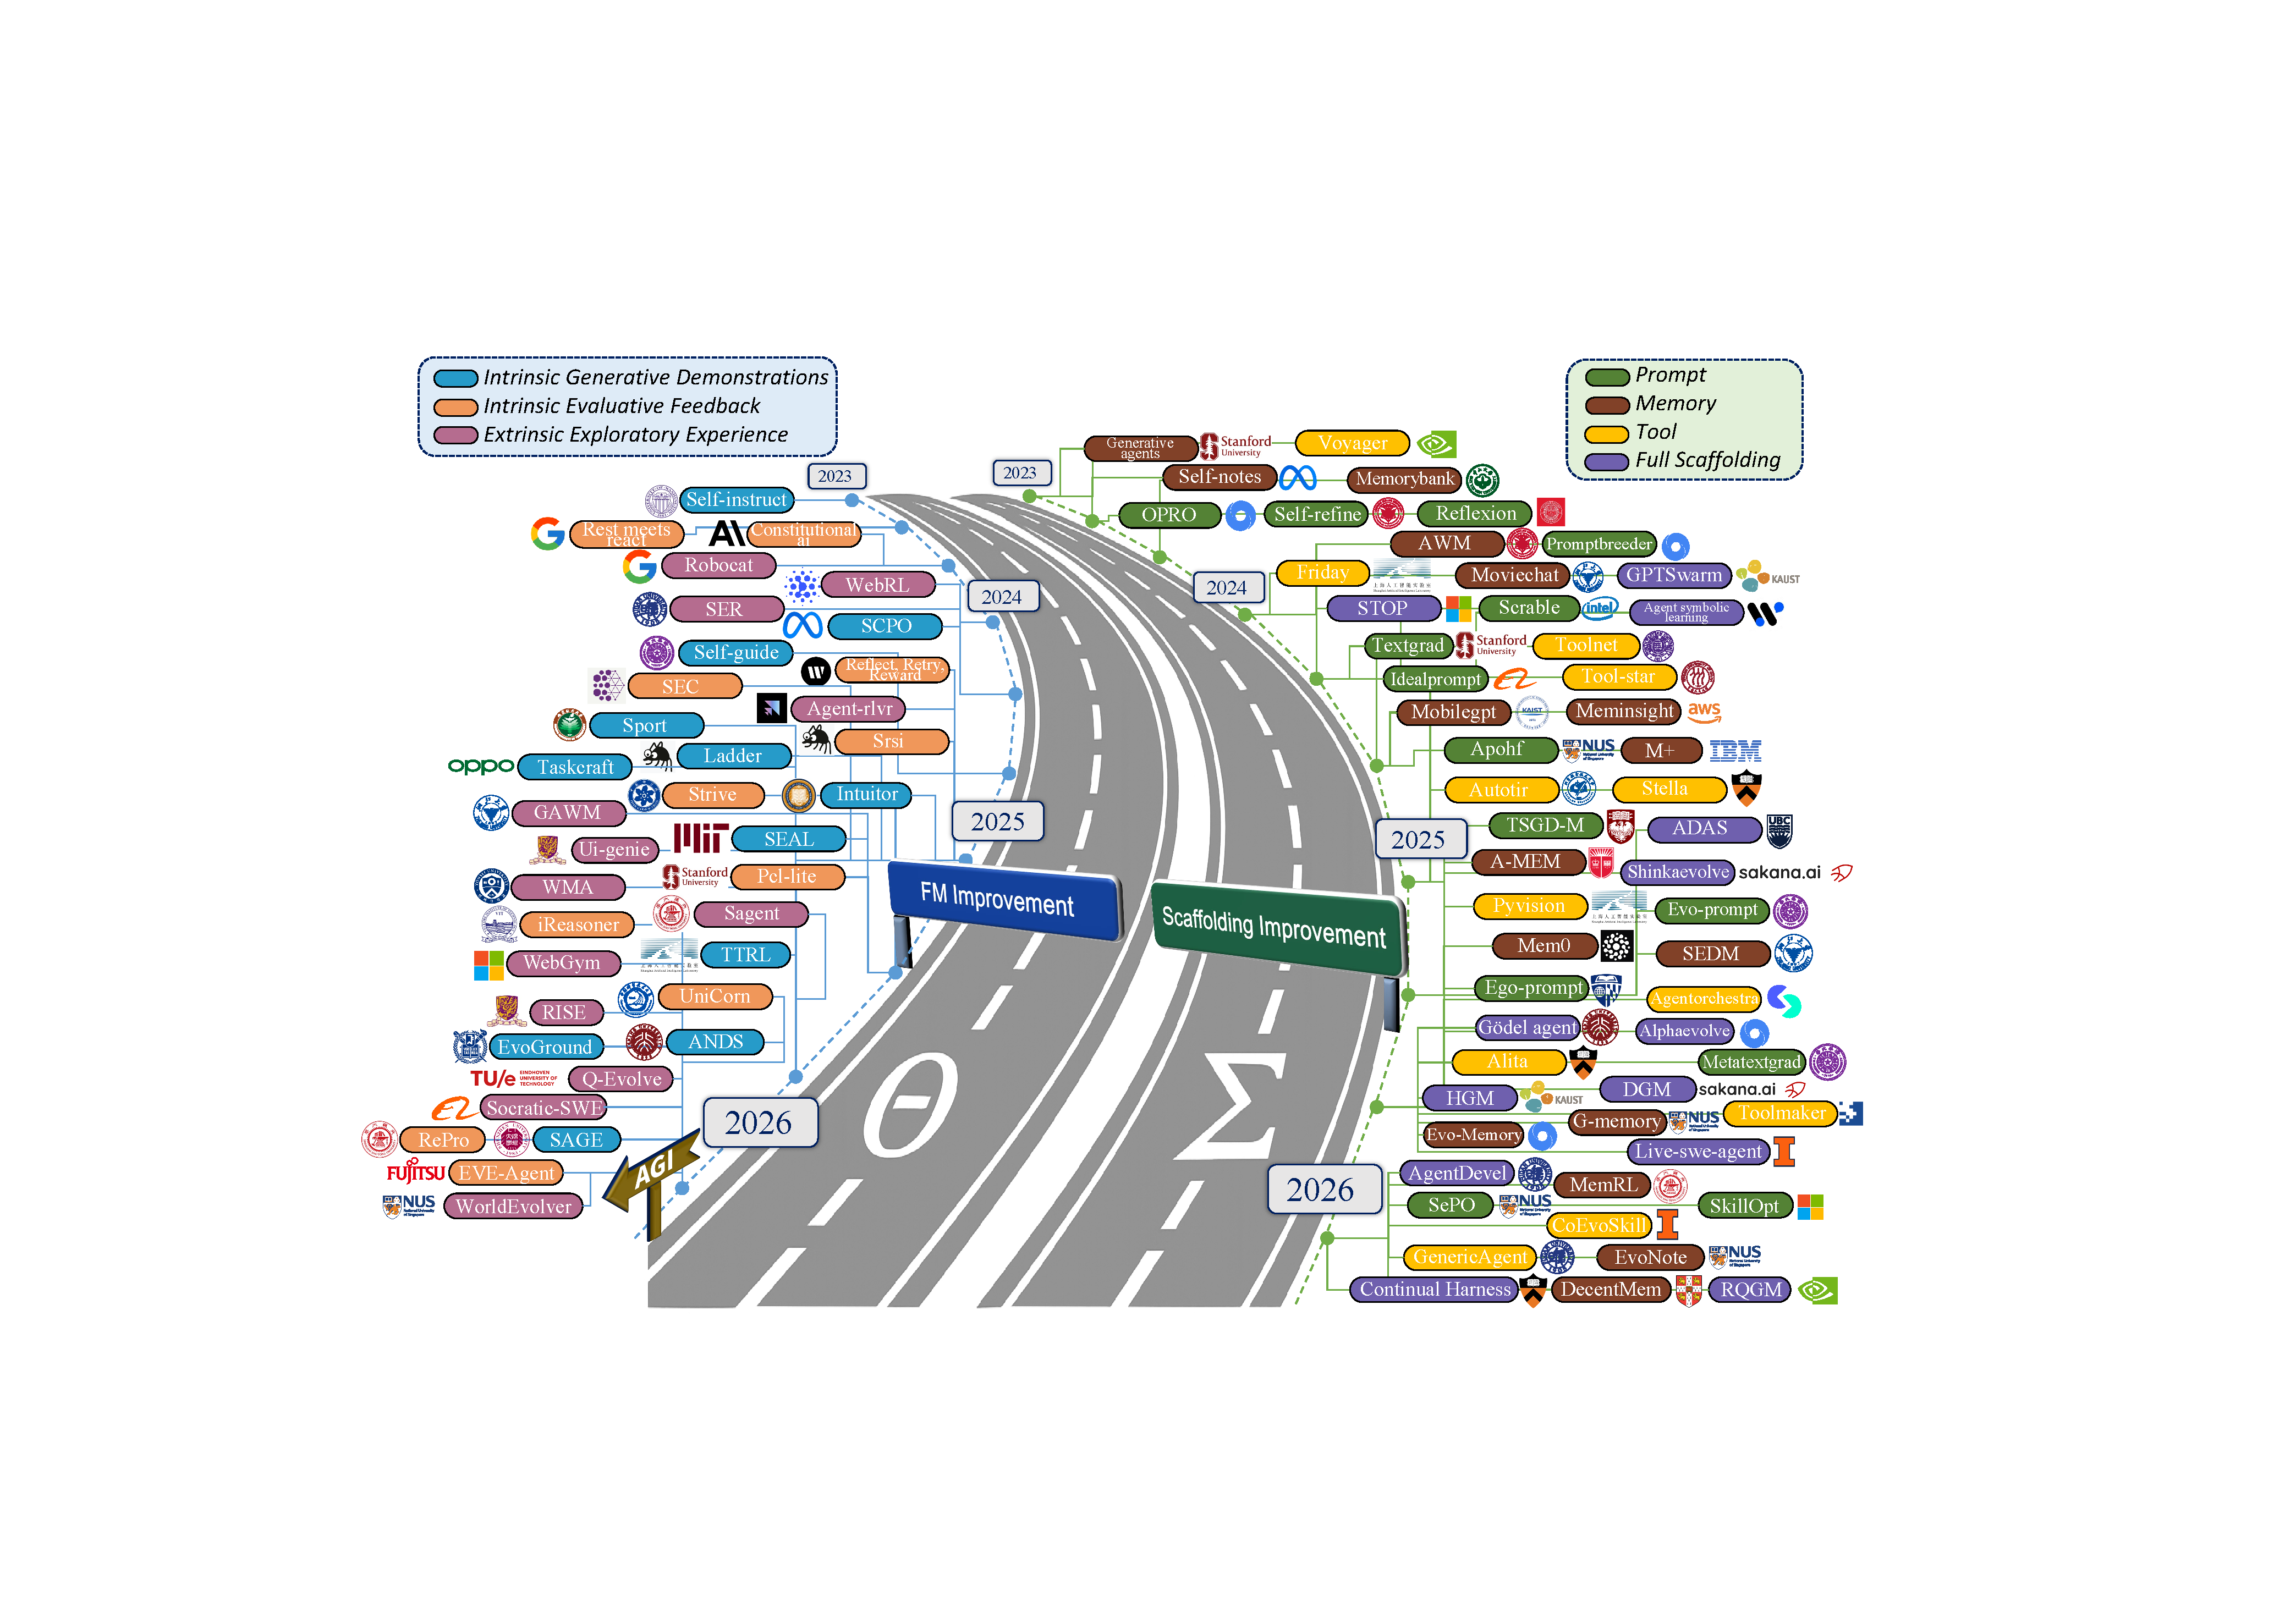
\includegraphics[width=1\linewidth]{fig/agent_timeline.pdf}
    \caption{Timeline and taxonomy of self-improvement in foundation-model-based agents (2023–2026). Representative works are positioned by publication year. The left lane denotes foundation-model improvement ($\theta$), while the right lane denotes scaffolding improvement ($\Sigma$). The AGI signpost highlights the field’s long-term aspiration toward increasingly general agentic intelligence.}
    \label{fig:agent_timeline}
\end{figure*}

